\documentclass[twosides]{EOSC350Lab} % 		DON'T SHOW ANSWERS
&\documentclass[twosides,showAnswers]{EOSC350Lab} % 	SHOW ANSWERS
\usepackage{graphicx}
\usepackage{caption}
\usepackage{subcaption}
\usepackage{changepage}
\usepackage{tikz}
\usepackage{nameref}

\newcommand{\TODO}[1]{{\color{red}#1}}

\newcommand{\ZipFile}{\href{https://www.dropbox.com/s/trn3huvlvb8nd3c/notebook.zip?dl=0}{Zip File~}}
\newcommand{\GPRMovie}{\href{http://www.eos.ubc.ca/courses/eosc350/content/2014/labs/Lab6/raypaths.html}{GPR Movie~}}
\newcommand{\GPGGPR}{\href{http://gpg.geosci.xyz/en/latest/content/GPR/index.html}{GPG: GPR Section}}
\newcommand{\SeismicRefractionChapter}{\href{http://gpg.geosci.xyz/en/latest/content/seismic/refraction/seismic_refraction_horizontal_layers.html}{GPG: Seismic Refraction Chapter}}

% === LAB INFO =================== %
\title{Lab 6: GPR}
\subtitle{Lab 6}
\TAname{Devin Cowan}
\TAemail{devinccowan@gmail.com}
\TAoffice{ESB 4021}
\labDate{October 24 \& October 26, 2016}
\dueDate{October 24 \& October 26, 2016}



% ====================================== %
% ======== DOCUMENT ==================== %
% ====================================== %

\begin{document}
\figdir{./Figures} % Figure directory

% ======== OVERVIEW AND INTRO MATERIAL ===== %
\begin{framed}



% ---------------- OVERVIEW ---------------- %
\section*{Overview}
During ground penetrating radar (GPR) surveys, an antenna is used to send a pulse of radiowaves into the Earth.
As the GPR signal propagates, it is reflected, transmitted and refracted at interfaces where the Earth's electromagnetic properties change.
Some of the GPR signal returns to the Earth where it is measured by a receiver.

%As in seismology, reflection and refraction events can occur when there are physical property contrasts in the subsurface. For GPR, the primary diagnostic %physical property is electrical permittivity. 

%GPR data are generally collected with a single source antenna and receiver antenna. We move along a line with fixed separation between source and receiver antenna so that we can obtain a line profile data, which is analogous to vertical section of the earth.

In this lab, you will consider the signals which propagate through a two-layer Earth.
For several models, you will also consider the ray paths which reach the receiver, and infer the signatures which present in the corresponding radargrams.
Finally, you will interpret radargram data collected at UBC.

% Other notes we may want to include: GRP generally collected with a single transmitter and receiver


% --------------- INSTRUCTIONS ------------- %
% \section*{Instructions}
% \label{sect:instructions}
% \begin{itemize}
% \item There are 15 questions labeled \textbf{Q}, some with multiple parts. Provide solutions for all of them.

% \end{itemize}


\subsection*{Running the iPython Notebook}
	For this lab, you will not have to write any code. You will only be running it.
	\begin{itemize}
		\item \emph{Shift + Enter} runs the code within the cell (so does the forward arrow button near the top of the document)
		\item You can alter variables and re-run cells by changing the values and doing \emph{Shift + Enter}
		\item If you want to start with a clean slate, restart the Kernel either by going to the top, clicking on \emph{Kernel: Restart}, or by \emph{esc + 00}
	\end{itemize}


% ------------ RESOURCES ---------------------- %
\section*{Resources}
\begin{itemize}
 	\item \GPGGPR 
 	%\item \GPRMovie
	\item \ZipFile containing the notebook
\end{itemize}

%To install it on your personal computer, refer to the instructions in the \nameref{sect:Appendix} of the lab.
\end{framed}
% ============================================================ %



\pagebreak


% ===========================START OF LAB ========================== %

%=================================
%	NEW SECTION: RAY PATHS
%=================================




\section*{Identifying the Ray Paths of GPR Signals}  % ================================= %
%\subsection*{Ray approach}
% LJH comments on Q1:
% Points to get across...
% - connection between physical properties and arrival times / ray paths
% 		- 2 direct rays, for both, the arrival times are described by linear relationships between offset and time with the slope being governed by the physical properties (velocity depends on relative permittivity.)
% 		- 1 refracted ray: the only place a critical refraction can be generated is at the surface
%		- reflections
%

Consider the model shown in Figure ~\ref{fig:profile_line}.
This model consists of three layers: air, layer 1, and layer 2.
The layers have relative permittivities $\epsilon_{r, air}$, $\epsilon_{r, 1}$ and $\epsilon_{r,2}$ respectively.
The distance between the source and the receiver is given by $x$.
The source and receiver antennas are oriented in $y$-direction.


		\begin{figure}[H]
			\centering 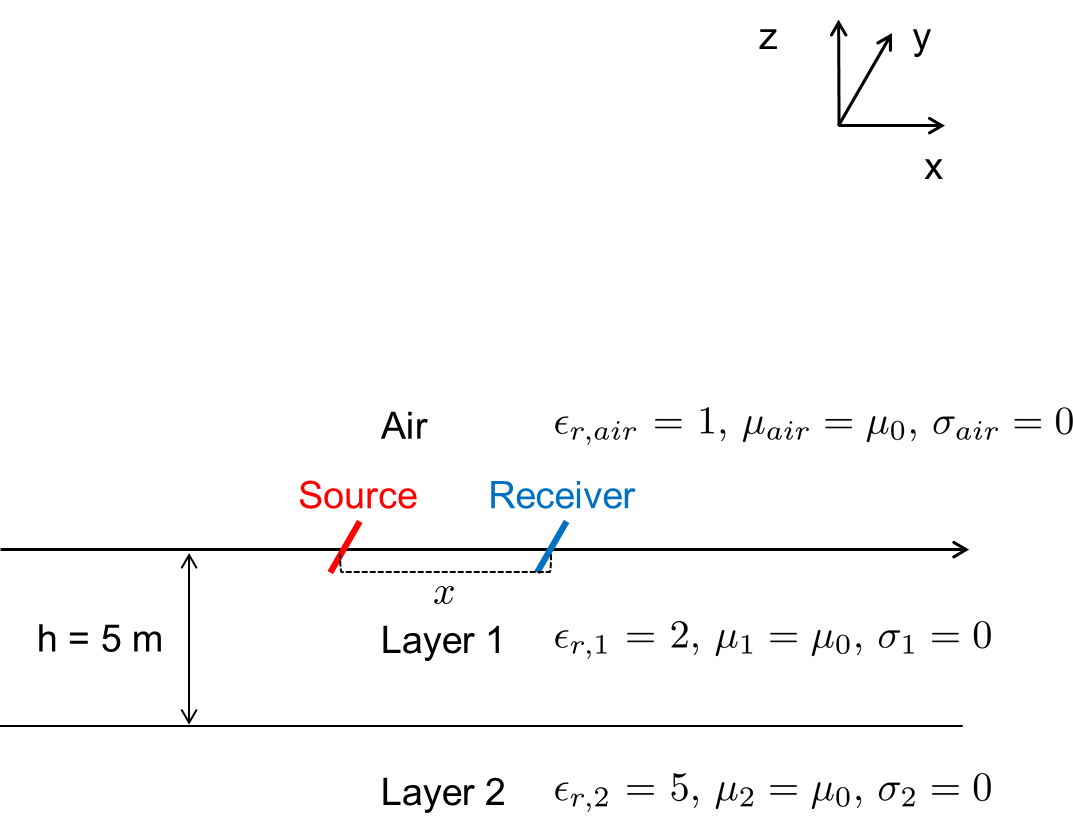
\includegraphics[width=0.75\textwidth]{Figures/profile_line.png}
			\caption{Conceptual diagram of GPR source antenna and receivers. }
			\label{fig:profile_line}
		\end{figure}




	  \question{For the model shown in Figure 1, there are a number of ways in which portions of the GPR wavefront (or waves) can reach the receiver. The different travel paths are called ray paths. Answer the following questions about GPR signals and ray paths.}


		\part{There are two direct paths which GPR signals can take from the transmitter to the receiver. Where do each of these waves propagate? Sketch the two ray paths on your own diagram below.}

			\answer{direct air wave and direct ground wave}

			\vspace*{50pt}

		\part{Which of the two direct signals will arrive first? Justify your answer by considering the physical properties of each medium. }

			\answer{air wave, $v = c/\sqrt(\epsilon_r)$ when $\mu_r = 1$, and $\epsilon_{r,air} < \epsilon_{r,1}$ always}

			\vspace*{60pt}

		\part{If the transmitter and receiver are separated by a distance $x$, what is the expression for the travel time for a direct wave?}

			\answer{t = x/v, where v = c/sqrt(eps)}

			\vspace*{60pt}


		\part{Suppose the operating frequency of the GPR system is 200 MHz. What is the spatial length (wavelength) of the GPR wavelet as it travels through the ground. Assume the ground has a relative permittivity of $\varepsilon_r = 4$. Sketch a typical wavelet below.}

		\answer{$\lambda = c / f_c \sqrt{\varepsilon_r}$ = 0.75 m} 

			\vspace*{80pt}



		\part{For layer 1, what is the smallest separation distance which two buried object could have and still be visible with a zero-off survey? Assume the objects are buried at a depth of 4 m. The operating frequency is still 200 MHz.}

		\answer{$D > \sqrt{\dfrac{V d}{2 f_c}}$ = 1.22 m}



\pagebreak

		\part{Plot the radargrams for the direct air wave and direct ground wave on  the t-x plot in Figure \ref{fig:txgrid}. Recall that we know the relative permittivity of air and that the relative permittivity of layer 1 is $\varepsilon_r$ = 4. }

			\begin{figure}[H]
				\centering 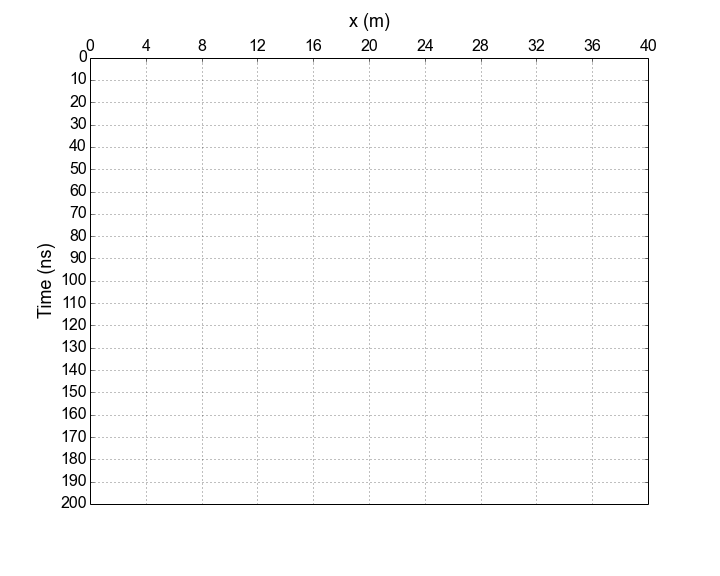
\includegraphics[width=1.\textwidth]{Figures/t_xgrid.png}
				\caption{T-X plot}
				\label{fig:txgrid}
			\end{figure}


		% LJH comment: wording? there are also multiples
		% Seogi comment: I think that this is fine in  this point whey they watch wave movie than they will recognize that.





		\part{When the GPR signal sent into the Earth reaches the interface between layers 1 and 2, some of it is reflected and some of it is refracted.}
\\\\
(i) Add the reflected ray path to your diagram in Question 1a.
\\\\
(ii) The formula for the travel time as a function of offset is given by $t = \sqrt{(x^2 + 4h^2)}/v_1$. Use this forumla to fill in the table below.
\\\\
(iii) Add the reflected wave signal to the T-X plot in Figure \ref{fig:txgrid}.}





	\begin{table}[H]
	\centering
		\begin{tabular}{| l | p{3cm}|}
		\hline
		\textbf{x (m)} & arrival time from the reflected wave at 1st interface (t) \\
		\hline
		0  &  \\[2ex]
		\hline
		1  &  \\[2ex]
		\hline
		2  &  \\[2ex]
		\hline
		4  &  \\[2ex]
		\hline
		8 &  \\[2ex]
		\hline
		16 &  \\[2ex]
		\hline
		24 &  \\[2ex]
		\hline
		\end{tabular}
	\end{table}


	\answer{67 ns, 67 ns, 68 ns, 72 ns, 85 ns, 126 ns, 173 ns}

		\part{For the geologic model we are considering, is it possible for there to be a critically refracted wave? Along which interface would the critically refracted wave travel if possible? Explain.}

			\answer{Yes. It would travel along the surface interface. Because $V_{air} > V_1$ always.}

			\vspace*{60pt}


		\part{Given that $\varepsilon_{air} = 1$ and $\varepsilon_1 = 4$, what is the angle for the critical refraction at the surface.}

			\answer{$\theta_c = \sin^{-1}(v_{1}/v_{air}) $ = 30 degrees}
			%\answer{$ Any ray path in which the critically reflected ray path  is translated toward the receiver will be valid$}

			\vspace*{40pt}

		\part{At what offset ($x_c$) will the critically refracted ray first be detected by receivers at the surface? Add the critically refracted wave to the T-X plot in Figure \ref{fig:txgrid}.}


			\answer{$x_c = 2h\tan\theta_c$ = 5.77 m}
			\vspace*{60pt}

%===========================================================
%		NEW QUESTION
%===========================================================


%%%%%%%% COMMENT: We just did the two layer case. Why should we do it again?!?!?!?!?


%
%
%	\question{Using the GPR widget (contained in the \ZipFile), we will estimate the unknown earth parameters,  $\epsilon_{r, 1}$, $h$ from the given data. For each of the following questions, record the value(s) you find. Before executing any of the codes be sure you have run ``Step 0: Import necessary packages.''}
%	%\TODO{DWO: definition in app: epsrL: relative permittivity for a linear arrival (direct or refracted wave
%	%epsrH: relative permittivity for a hyperbolic arrival (reflection))}
%
%		\part{Identify the direct air wave in the data and fit the arrival tmes with a straight line (blue) by adjusting epsrL and tinterpL. Record these values. }
%
%		\answer{interpL = 15, epsrL = 1}
%
%			\vspace*{40pt}
%
%		\part{Identify the direct ground wave and fit the arrival times with a straight line (blue) by adjusting epsrL and tinterpL. Record these values.}
%
%		\answer{interpL = 15, epsrL = 9}
%
%			\vspace*{40pt}
%
%		\part{Identify the reflected wave from the interface between the first and second layer and fit it with a hyperbola (red) by adjusting tinterpH and epsrH. Since the reflected wave travels through the first layer, you may use the relative permittivity you found for the direct ground wave for epsrH. Record the estimated tinterpH and esprH values. }
%
%		\answer{interpH = 115, epsrH = 9}
%
%			\vspace*{40pt}
%
%		\part{What is the velocity of the wave in the first layer?}
%
%		\answer{0.1 m/ns}
%
%			\vspace*{40pt}
%
%		\part{What is the thickness of the first layer, $h$?}
%
%		\answer{$d = \dfrac{Vt}{2} = 0.1 m/ns \times 115 ns /2$ = 5.75 m}
%
%			\vspace*{40pt}


%=================================================
% NEW SECTION: DRAWING RAY PATHS
%=================================================


\section*{Sketch ray paths on a profile line}

% LJH Comment: This is where we could include some info in Huygen and Fermat principals if we want to

% Seogi comment: Let's not put those concepts in this time. It should be tied with Doug's lecture I guess, so next time.

% Rays are defined as the normal to the wavefronts as shown in Figure ~\ref{fig:ray}.

%The geometry of a wavefront is governed by Huygens’ principle and the geometry of ray-paths is governed by Fermat's principle. {\color{red} @ SEOGI: a bit of explination here? }
%LJH comment: there are a lot of concepts being thrown at them in this sentence, we should given them some definitions...

	% \begin{figure}[H]
	% 	\centering 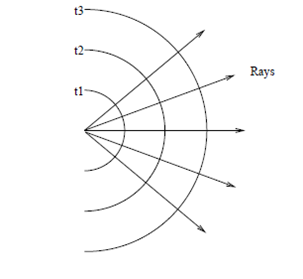
\includegraphics[width=0.3\textwidth]{Figures/ray.png}
	% 	\caption{Conceptual diagram of wavefront and ray. }
	% 	\label{fig:ray}
	% \end{figure}
	% \question{What is Huygens' principle? }

	% 		\answer{...}

	% 		\bigskip
	% 		\bigskip

	% \question{What is Fermat's principle?}

	% 		\answer{...}

	% 		\bigskip
	% 		\bigskip

In this section, we sketch ray paths for the GPR survey configurations and models provided. By drawing the ray paths, we can then infer the features we would expect to see in the corresponding radargram.
% and assume the following set-up:

% LJH comment: Is the term "minimum ray path" going to the confusing?
% Seogi comment: I am not sure. We can introduce briefly in the lab.
%\begin{itemize}
%	\item We only consider the reflected rays from the objects (anticline, pipe and slab)
%	\item For zero offset, the reflections will be at normal incidence.
%	\item We only consider the minimum ray path. %LJH comment: this may be a confusing statement
%	\item Since it is reflection, angular relationship of incident and reflected ray is governed by Snell's law.
%\end{itemize}
%For the GPR survey configuration, we have a source antenna and a receiver antenna. Here we consider the situation where their separation  is zero.

	\question{Consider the thick slab model in Figure \ref{fig:slab}. Let the black dots represent the Tx-Rx locations for a {\bf zero offset} configuration.}

		\part{Sketch the reflected ray paths for the slab model given below. Recall that rays which reflect off a point will reflect in all directions.}
			\begin{figure}[H]
				\centering 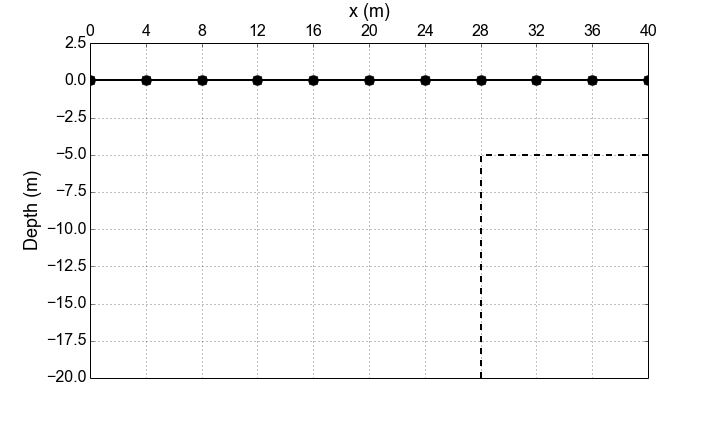
\includegraphics[width=0.8\textwidth]{Figures/wall.png}
				\caption{Ray paths for the slab model.}
				\label{fig:slab}
			\end{figure}

		\part{If the slab was very thin (a horizontal pancake), would the ray paths change? Why?}

		\answer{No. None of the reflected waves from the vertical face will reach a receiver.}

				\vspace*{40pt}

\pagebreak


		\part{Based on ray paths you drew on Figure \ref{fig:slab}, sketch the corresponding radargram on the figure below. You will first need to determine the top-layer velocity. This can be done by looking at the arrival time to depth conversion between Figures \ref{fig:slab} and \ref{fig:t_xgrid_sketch}. Assume that it takes 200 ns for a reflected signal at 20 m depth to return.}
		%Mark time arrivals for each source and receiver antenna pair at center location of them.}
			\begin{figure}[H]
				\centering 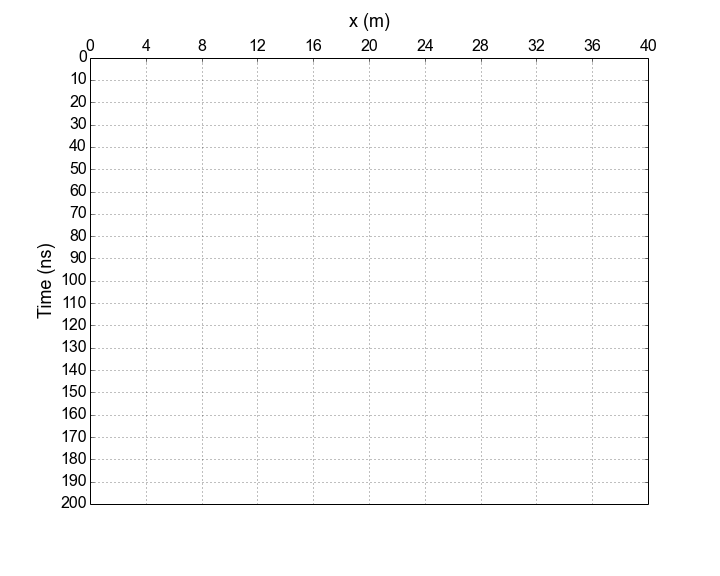
\includegraphics[width=0.8\textwidth]{Figures/t_xgrid.png}
				\caption{Arrival times for the slab model}
				\label{fig:t_xgrid_sketch}
			\end{figure}



%============================
%	SYNCLINE MODEL
%============================


	\question{Consider the concave interface in Figure \ref{fig:syncline}. Once again, we will use a zero offset survey configuration.}


		\part{Sketch the reflected ray paths for the interface given below when the GPR unit is at x=8, x=16 and x=20m}
			\begin{figure}[H]
				\centering 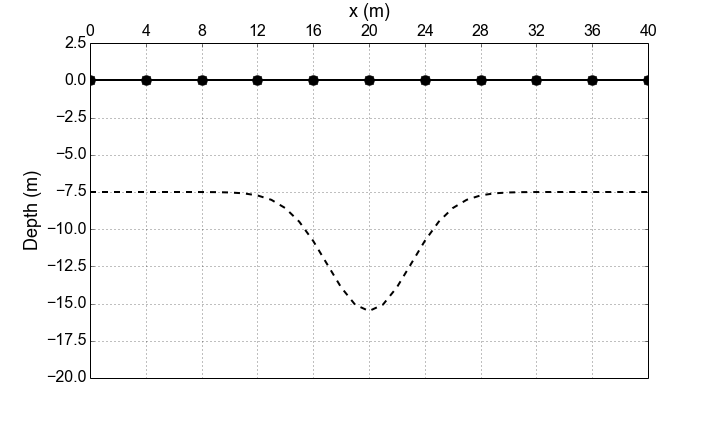
\includegraphics[width=0.8\textwidth]{Figures/anticline.png}
				\caption{Ray paths for the syncline model}
				\label{fig:syncline}
			\end{figure}


		\part{Why might it be more difficult to infer the shape of this interface from radargram data?}

		\answer{Because we will see multiple reflected signals for the same interface.}

	\vspace{40pt}

%		\part{Based on zero-offset ray paths you drew, sketch the radargrams at the receiver locations.}
%		%Mark time arrivals for each source and receiver antenna pair at center location of them.}
%			\begin{figure}[H]
%				\centering 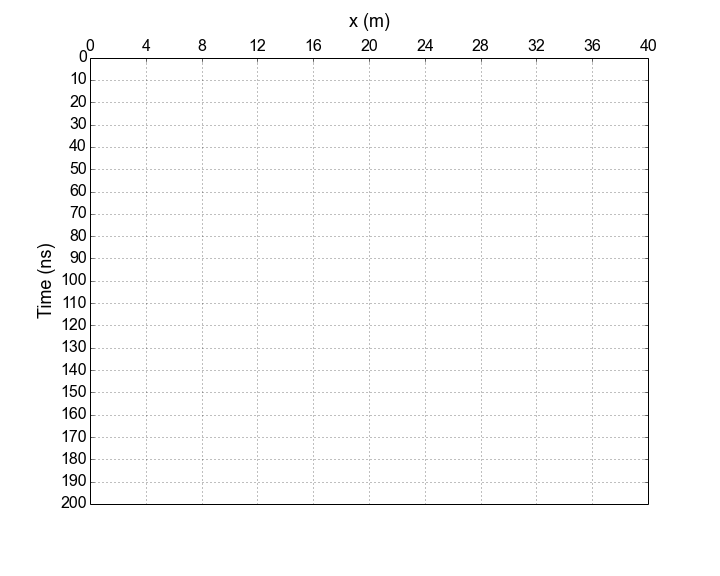
\includegraphics[width=0.8\textwidth]{Figures/t_xgrid.png}
%				\caption{Radargrams for the syncline model}
%				\label{fig:t_xgrid_sketch_2}
%			\end{figure}



% \section*{Sketch responses}
% Based on ray paths that you draw for three models, now sketch arrival time of those rays at receiver locations. You need to mark time arrivals for each source and receiver antenna pair at center location of them.
% 	\question{A pipe model}
% 		\begin{figure}[H]
% 			\centering 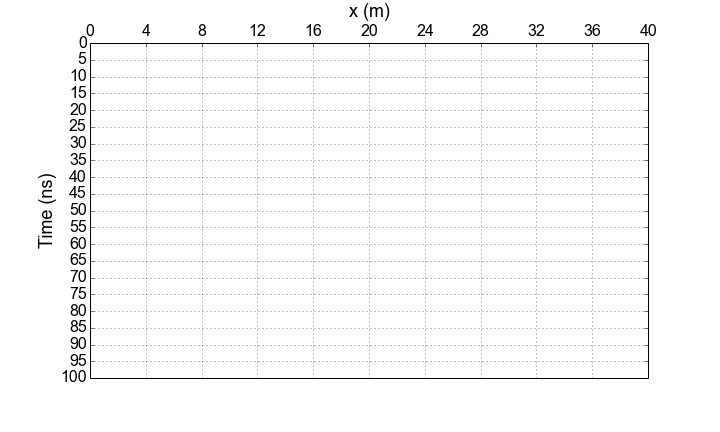
\includegraphics[width=0.7\textwidth]{Figures/t_xgrid_sketch.png}
% 			\caption{}
% 			\label{fig:t_xgrid_sketch}
% 		\end{figure}

% 	\question{A slab model}
% 		\begin{figure}[H]
% 			\centering 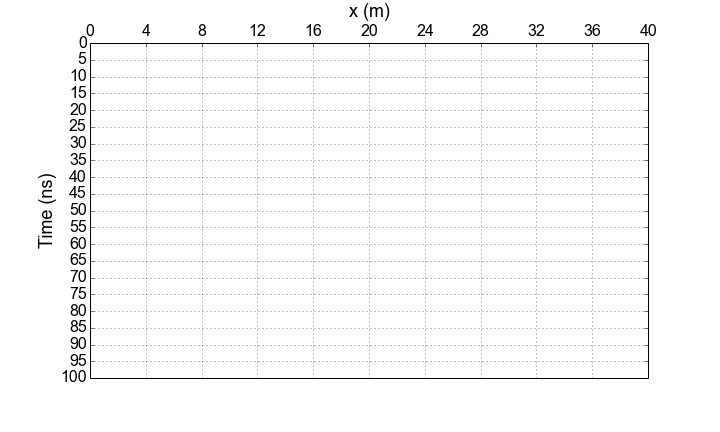
\includegraphics[width=0.7\textwidth]{Figures/t_xgrid_sketch.png}
% 			\caption{}
% 			\label{fig:t_xgrid_sketch}
% 		\end{figure}

% 	\question{An anticline model}
% 		\begin{figure}[H]
% 			\centering 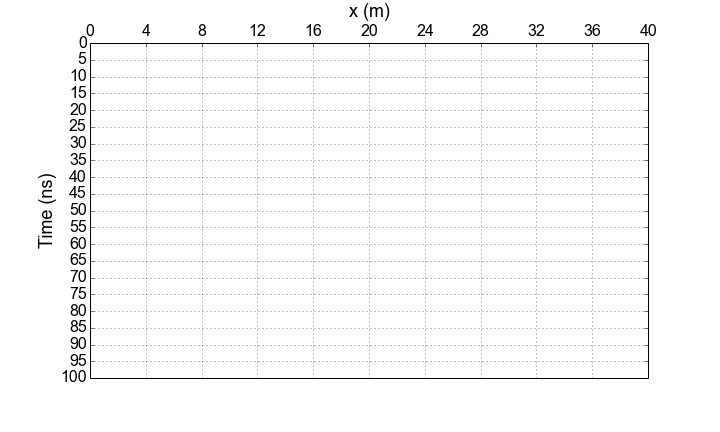
\includegraphics[width=0.7\textwidth]{Figures/t_xgrid_sketch.png}
% 			\caption{}
% 			\label{fig:t_xgrid_sketch}
% 		\end{figure}


%\TODO{DWO: As good as this section is, I think we need to omit questions here. Leave this functionality in the app. Can we use the app for the team TBL? Issues of frequency vs penetration. See Overmeeren. Also, we don't want to lose the associated questions. Any suggestions for how to archive them so they don't get lost?}


%\section*{Effect of electrical conductivity in GPR}
%\section*{EM wave velocity and depth of investigation}

%To simplify the GPR problem, we previously assumed that there was no conductivity effect. However, in practice, this is not true. Some earth materials can have quite high conductivity values. In this case, assuming that we do not have a conductivity effect does not make sense. In addition, this conductivity effect can be advantageous in certain circumstances. For example, we can differentiate fresh and saline water boundaries, which is useful to map sea water intrusions, because saline water is much more conductive than fresh water. In this section, we investigate the effect of conductivity in GPR.
%\subsection*{EM wave velocity and depth of investigation}

%/question{Background checks for EM wave velocity:}

%	\part{What is the EM wave velocity as a function of relative permittivity ($\epsilon_r$) and velocity of light ($c$).}
%		\vspace*{60pt}

%	\part{What is the EM skin depth as a function of relative permittivity ($\epsilon_r$) and conductivity ($\sigma$).}
%%		\answer{$\delta=\frac{5.31 \sqrt{\varepsilon_r}}{\sigma}$}

%	\part{What are we assuming in the above equations?}
%		\vspace*{60pt}

%	\question{When this condition is not verified, there is an additional frequency dependency in addition of the previous parameters. Use the app "interact in step 2 of the ipython notebook to help you answer the following question. }
%	 	\part{which parts of the graphs correspond to the GPR regime?}
%	 	\vspace*{60pt}

%		\part{ How would you describe the frequency dependency on velocity? What is the effect of conductivity on velocity as a function of frequency? }
	%\part{Do you recognize that there are more material properties, which affects EM wave velocity? Put two more factors, which affects EM wave velocity.}
%		\vspace*{60pt}

%		\part{ How would you describe the frequency dependency on skin depth?}
%		\vspace*{60pt}

%\question{Next we use Step2 of the GPRWidget to explore EM wave velocity.}

%	\part{Run this widget, then see the left plot, which shows the velocity of the EM wave. Here the $x$ and $y$ axes are frequency (Hz) and velocity (m/s), respectively. Observe how the EM wave velocity changes as a function of frequency, and provide a description of the frequency effect. Record the frequency range where EM wave velocity is independent of frequency.}
%		\vspace*{80pt}

%	\part{Fix conductivity (sigma in the widget) to $10^{-4}$, then change relative permittivity (epsr in the widget) from $1-80$. Record your observations. }
%		\vspace*{60pt}

%	\part{Fix relative permittivity (epsr in the widget) to 1, then change conductivity (sigma in the widget) from $10^{-8}$-$10^0$ S/m. Write down your observations. }
%		\vspace*{60pt}

%\subsection*{Attenuation of EM waves}
%\question{Background checks for EM wave attenuation:}

%	\part{How is skin depth approximated for the cases where $\frac{\sigma}{\omega\varepsilon} >>1 and <<1$ ?}
%		\vspace*{60pt}

%	\part{What affects the attenuation of EM waves? Provide two factors. }
%		\vspace*{60pt}

%	\part{Based on the definition of skin depth, let us assume that we have three GPR instruments, which use 25, 50 and 100 MHz frequencies. Which one provides you the largest depth of investigation?}
%		\vspace*{60pt}	

%\question{Now we will use Step2 of the GPRWidget to explore EM wave attenuation}

%	\part{Run this widget, then see the right plot, which shows the skin depth of an EM wave. Here the $x$ and $y$ axes are frequency (Hz) and skin depth (m), respectively. Observe how skin depth changes as a function of frequency, provide a description of this relationship. Record the frequency range where skin depth is independent of frequency.}

%	\part{Fix conductivity (sigma in the widget) as $10^{-4}$, then change relative permittivity (epsr in the widget) from $1-80$. Write down your observations. }

%	\part{Fix relative permittivity (epsr in the widget) as 1, then change conductivity (sigma in the widget) from $10^{-8}$-$10^0$ S/m. Write down your observations. }

%\subsection*{Conductivity effects in  EM wave}

%\question{In (Overmeeren, 1994), the author said ``In practice, georadar is unfit for use in areas where the soil resistivity is less than 100 $\Omega$-m; this is the case in clayey and silty formations and in brackish and saline ground water environments''. In addition, they provide a table, which shows EM wave velocity and attenuation in various materials, as shown in Figure \ref{fig:table_gpr}. Answer following questions: }

%	\begin{figure}[H]
%		\centering 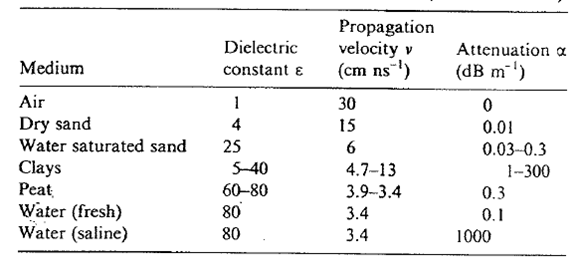
\includegraphics[width=0.7\textwidth]{Figures/table_gpr.png}
%		\caption{Characteristic values of physical properties of media important for georadar (Davis and Annan 1989; Hänninnen 1992).}
%		\label{fig:table_gpr}
%	\end{figure}

%	\part{Use the SigmaEffectWidget; set your relative permittivity to 4, which is similar to dry sand, then record the skin depth of a medium with a conductivity of $10^{-2}$ S/m at 100 MHz. Record the EM wave velocity as well. }

%	\answer{About 1 m.}
%		\vspace*{60pt}

%	\part{Now we decrease the conductivity value to $10^{-3}$ S/m. Leave the other parameters fixed. Record the skin depth and EM wave velocity, and compare them with the previous case where the conductivity value was $10^{-2}$ S/m.}

%	\answer{About 10 m.}
%		\vspace*{60pt}

%	\part{In Figure \ref{fig:table_gpr}, the author states that the EM wave velocities of fresh and saline water are the same (3.4 cm/ns). Evaluate this statement using the SigmaEffectWidget. Use $10^{-2}$ and $10^{0.5}$ S/m for the conductivity values of fresh and saline waters, respectively, and 100 MHz frequency.}

%		\vspace*{60pt}








%====================================
% NEW SECTION: INTERPRETING FIELD DATA
%====================================


\section*{Interpretation of Field Data}
In this section, we will interpret field collected GPR data collected at the University of British Columbia. Applications in the GPRWidget will help you answer subsequent questions. {\bf For all remaining questions, we will only be using Step 4a and Step 4b in the GPRWidget.}
% LJH comment: can we give a bit more back-story on why this data set was collected? What motivated it?
% Seogi comment: That's good idea, but actually I don't know. So, we need to ask Doug.



%===========================================
% QUESTION IS EFFECTIVELY THE SAME AS Q2
%===========================================


%\question{The data shown in Figure ~\ref{fig:ubc_GPRcmp_coord} were collected using the common midpoint survey configuration. In this case, the smallest offset distance was 2.4 m (not 0 m). For the following questions, use Steps 2-4 of the GPR widget.}
%
%		\begin{figure}[H]
%			\centering 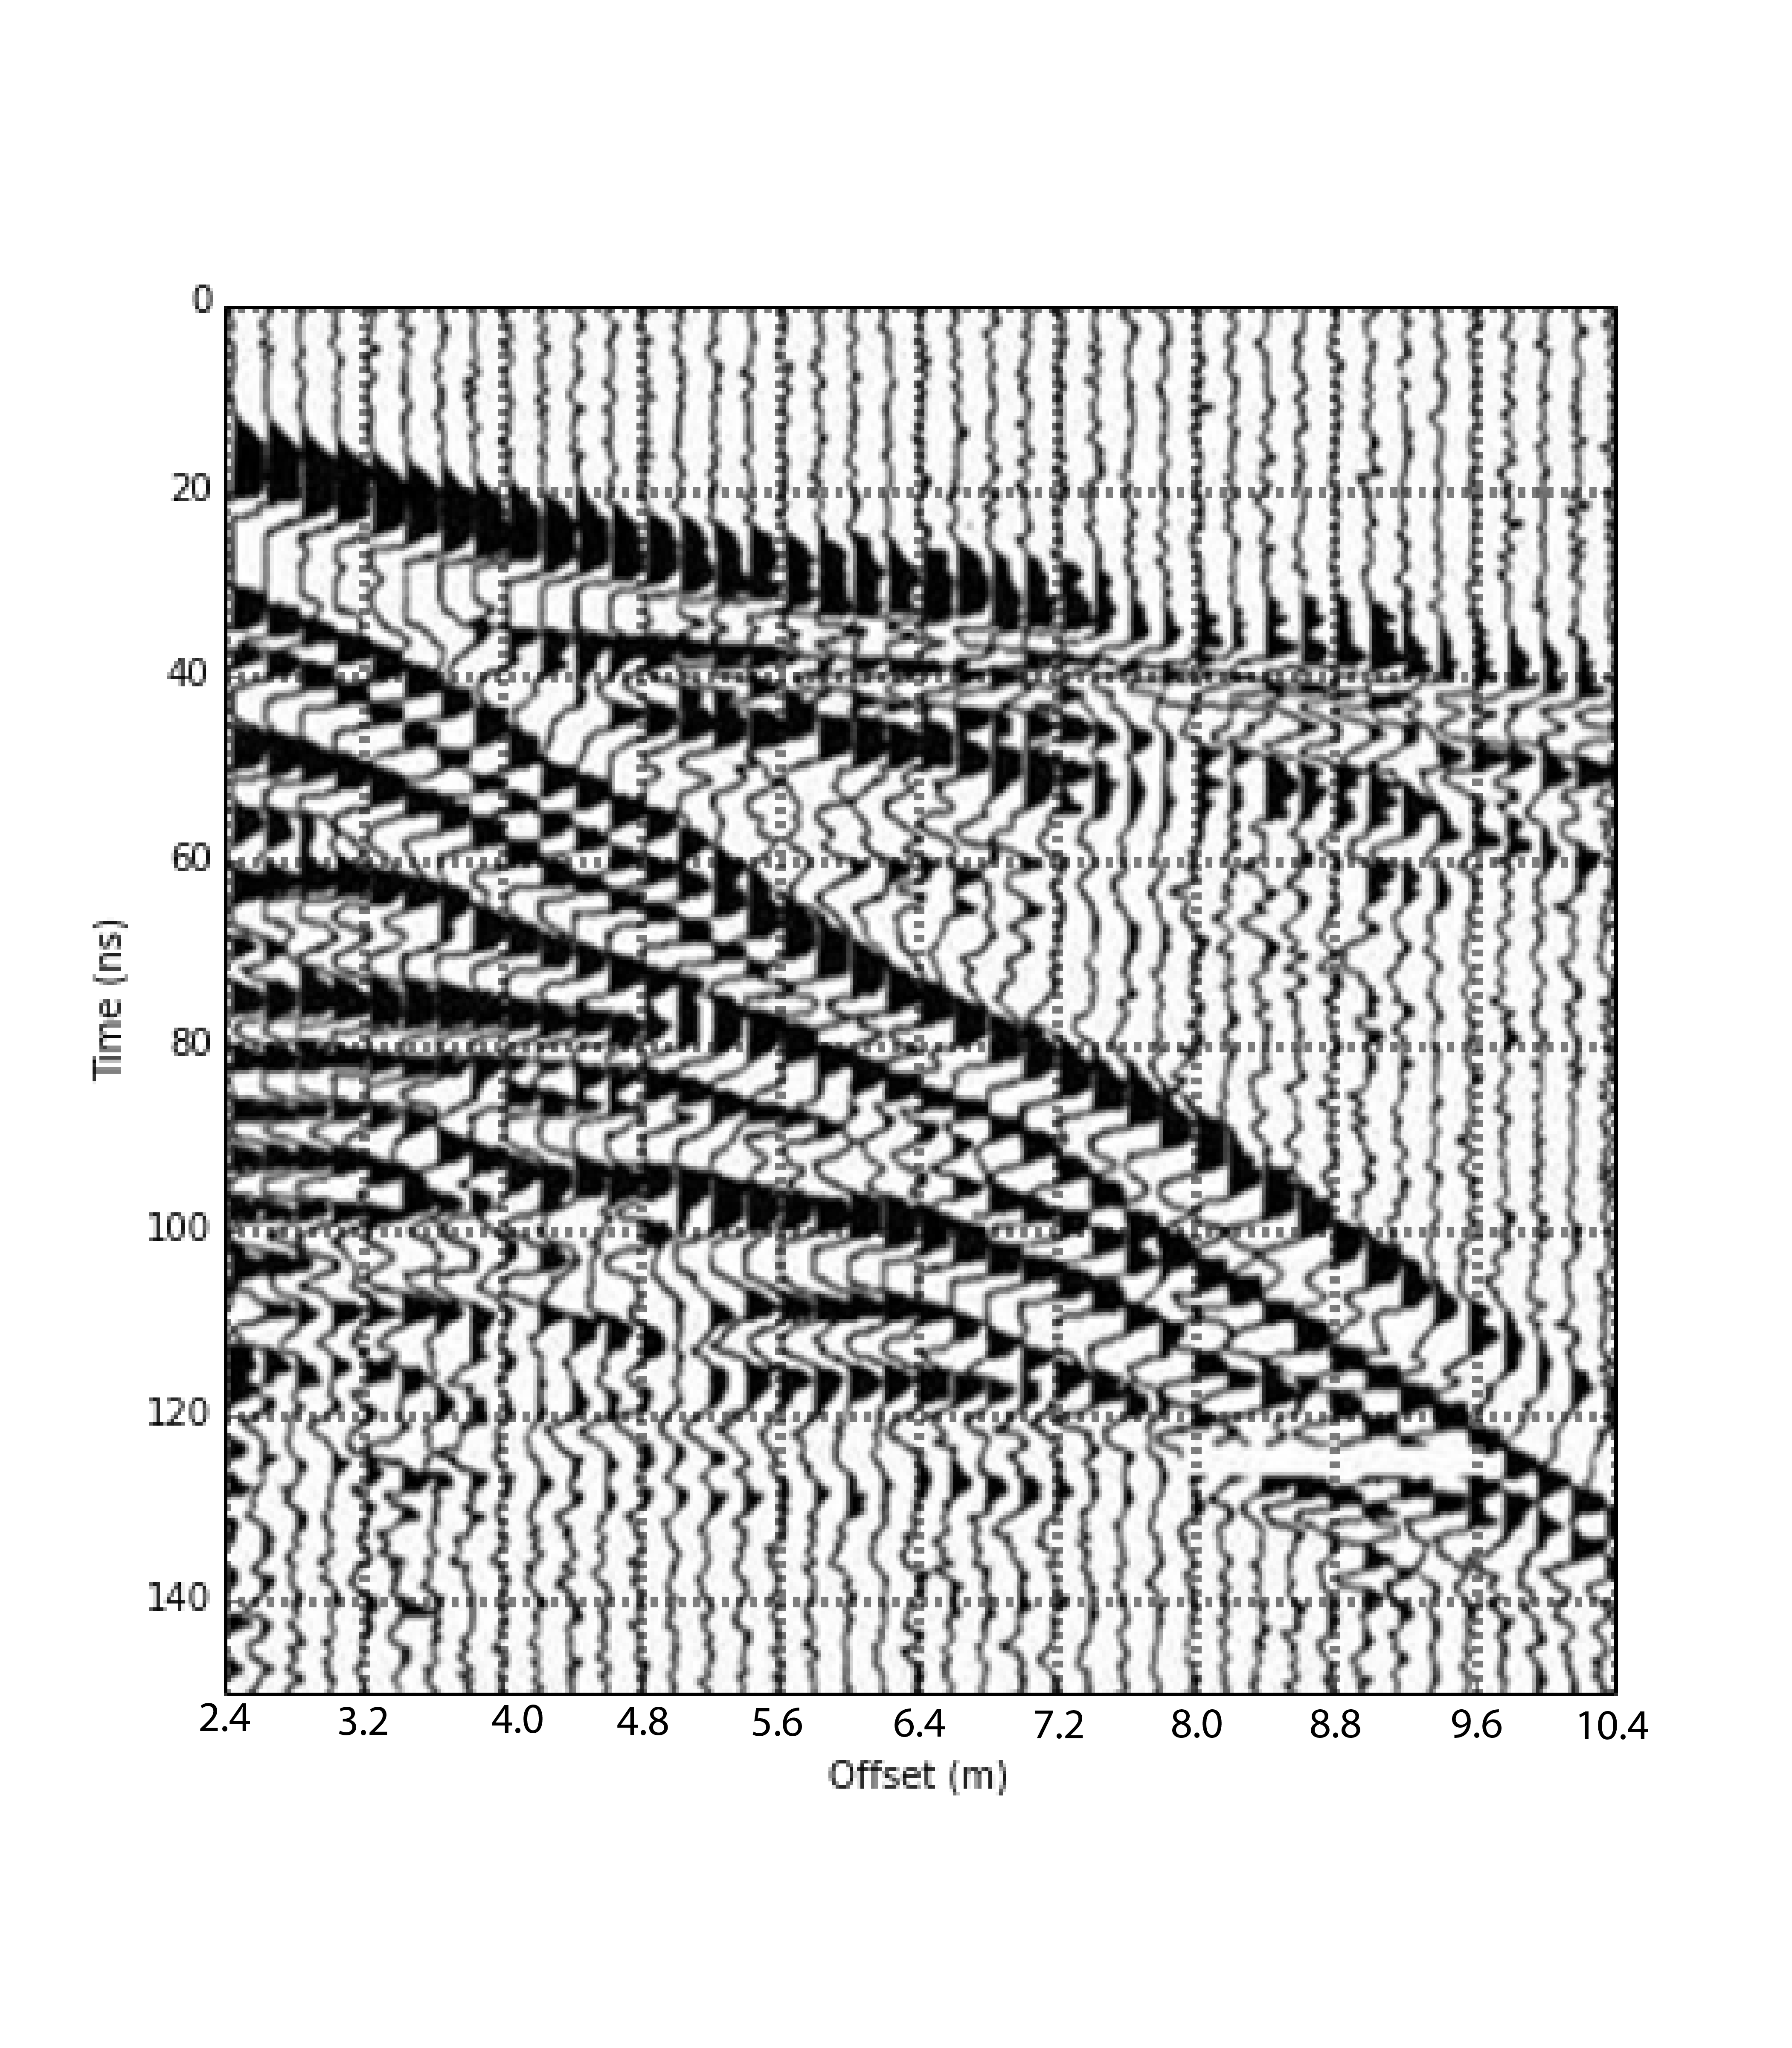
\includegraphics[width=0.7\textwidth]{./Figures/ubc_GPRcmp_coord.png}
%			\caption{Common Midpoint data collected by UBC. }
%			\label{fig:ubc_GPRcmp_coord}
%		\end{figure}
%
%		\part{Pick out the air wave and estimate its velocity.}
%
%		\answer{}
%
%			\vspace*{40pt}
%
%		\part{Identify the direct ground wave and estimate its velocity.}
%
%		\answer{}
%
%			\vspace*{40pt}
%
%			\part{The radargram is not easily interpreted but there is a distinct flattening out of the reflections at small offsets. This is characteristic of a reflection hyperbola. Pick a possible candidate for this reflective event and extrapolate back to zero offset. What is the depth of the layer that gives rise to this reflection?}

% LJH comment: I am a bit confused by the second sentence in this question (the one I commented out), are you referring to figure 12 or 13?


%====================================================
%	NEW QUESTION
%====================================================


	\question{Consider the radargram data shown in Figure ~\ref{fig:ubc_GPRdata_coord}. These data were collected using a zero offset survey. Let us assume we know there are three different types of objects present:}
		\begin{itemize}
			\item Layered interfaces 
			\item Buried pipes
			\item A concrete utility casing
		\end{itemize}

		\begin{figure}[H]
			\centering 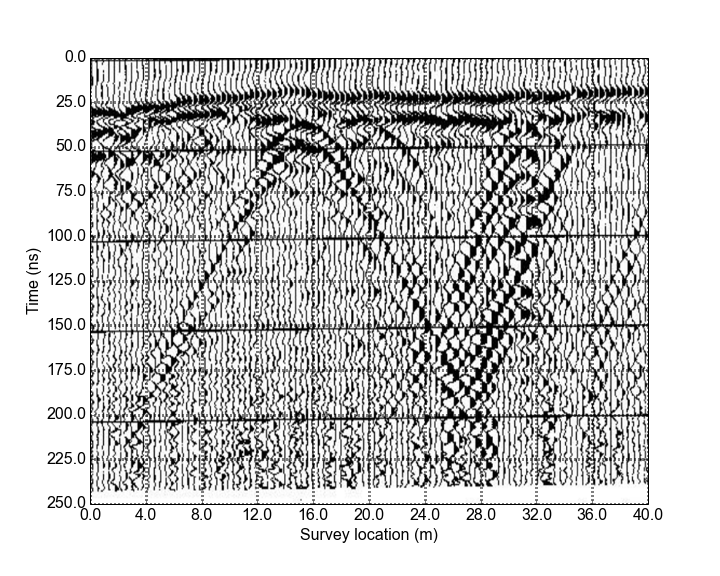
\includegraphics[width=0.8\textwidth]{Figures/ubc_GPRdata_coord.png}
			\caption{Common offset profile collected by UBC}
			\label{fig:ubc_GPRdata_coord}
		\end{figure}
	%Common mid point survey shown in Figure ~\ref{fig:ubc_GPRcmp_coord} was collected at the location $x=$ 2 m shown in Figure ~\ref{fig:ubc_GPRdata_coord}.



	\part{On Figure \ref{fig:ubc_GPRdata_coord}, identify the signatures attributed to buried pipes on the radargram (there are two).} 

\vspace{30pt}


	\part{Using the GPRWidget, fit the left-most signature by adjusting the parameters provided: epsr (relative permittivity), h (distance of the pipe center from the surface), xc (the pipe center location), r (radius of the pipe). Record the parameters you used.
		}

			\answer{epsr = 23, h = 1.8, xc = 15.6, r = 1.2}
			\vspace*{40pt}	


	\part{Now fix the radius and depth to the pipe as r = 0.5 m and h = 1.5 m, respectively. Are you able to fit the left-most pipe by adjusting only epsr and xc? Write down the relative permittivity and centre location which gave you the best fit.}


	\answer{epsr = 23, xc = 15.6}

	\vspace{40pt}
		

	\part{Try using parameters: epsr = 28, h = 1.7, xc = 15.4 and r = 0.7. Do these parameter value fit the signature from the pipe reasonably well? Therefore, is there a unique set of parameter values which fit the data or is the solution "non-unique"?}


	\answer{Yes. The solution is non-unique.}

	\vspace{40pt}




\part{Based on your answer to the previous question, answer the following. (i) Is the set of parameter values which fit the data always always correspond to the correct answer? (ii) If a set of parameter values does not fit the data, can it be ruled out as a potential solution?}


	\answer{No. Yes.}

	\vspace{40pt}





\part{Set the parameter values to: epsr = 28, h = 1.5, xc = 15.4 and r = 0.4. Now slowly increase the radius of the pipe to 3 m and examine how the curve is changing. Note that as you increase the radius of the pipe, it stops being a point reflector. (i) Is the slope of the "tails" of hyperbolic signature changing as you increase the radius? (ii) Can we use the slope to estimate the top layer velocity if the pipe is thick?}


	\answer{No. Yes.}



	\vspace{60pt}







		\part{On Figure \ref{fig:ubc_GPRdata_coord}, draw a line where you are observing the reflection from a layer boundary. Using the parameters from your answer in {\bf b)}, estimate the top layer velocity and approximate the depth to the chosen reflector. Show the equations you used.}
		

			\answer{$V = c/\sqrt{\varepsilon_r} \sim $ .063 m/ns. $D = 1/2 \times 25ns \times 0.63 m/ns \sim$ 7.9 m.}


			\vspace*{40pt}


			





		

		% LJH comment: can we be more specific about the last sentence? What are you expecting them to put down?
		

%	\part{Compute the velocity of the GPR signal using the estimated relative permittivity. Compare this velocity with one that you computed in Question 5b (based on the CMP gather shown in Figure ~\ref{fig:ubc_GPRcmp_coord}. The CMP gather data were acquired near the location of the profile line data). How do the velocities compare? Can you find a relative permittivity for the top layer that was satisfactory for both data sets?  If you can't, can you suggest any reason for the discrepancy or could you reconsider any of your analysis to find a relative permittivity value?}
%
%			\answer{.I got epsr=11 for the CMP gather and epsr=25 for the pipe. The direct wave for the CMP gather is sensitive to the velocity right at the surface. In the COG (Common Offset Gather) the waves are travelling through the upper meter or more of the ground. If the moisture level is increasing with depth then so will epsr. This might be a possible explanation. ..}
%			\vspace*{60pt}




		\part{Identify the response due to the large concrete casing. Label where you think the concrete casing is on Figure \ref{fig:ubc_GPRdata_coord}. Hint: the shape of the signature should be {\bf very} similar to that of the slab in {\bf Q2}.}



		\vspace{30pt}

		\part{Using the GPRWidget, fit the signature you chose by adjusting the parameters for the slab. Record the parameters that you find.}

			\answer{...}
			\vspace*{40pt}




	\part{When the transmitter and receiver are located at roughly 30 m along the profile line, notice that a signal persists over most of the observation times. Both the pipes and the concrete casing are strong conductors (great reflectors). (i) If one of the pipes is very near to the concrete casing, what might be causing this signal? (ii) Did the effects of this signal make it more difficult to locate the left-most margin of the concrete casing?}

	\answer{Ringing. Yes.}
			\vspace*{40pt}




% \section*{Appendix}
% \label{sect:Appendix}
% \subsection*{How to get the iPython Notebook}
% If you want to run ipython notebook in your home, first you need to download whatever python package mananger, for instance Canopy or Ananconda. We provide you the instructions for Canopy.
% \begin{enumerate}
% 	\item{Download \href{https://store.enthought.com/downloads/}{Canopy}. The basic version is free.}
% 	\item{Open up the download and install. Follow the instructions. It will install the required packages and set the necessary paths on your computer.}
% \end{enumerate}

\end{document}
% ========================================================= %
